\chapter{Design}
\label{design}

\section{Protocol Design}

\subsection{Protocol Overview}

\begin{figure}[!h]
    \begin{center}
        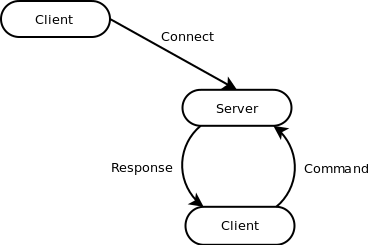
\includegraphics[scale=0.65]{chapter2/diagrams/protocol_high_level.png}
        \caption{The exchange of messages between a client and the server}
        \label{highLevelDia}
    \end{center}
\end{figure}

Gim uses a client-server architecture, where one computer (known as the Sever) acts as a central point which other computers (the Clients) connect. The clients do no communicate directly with each other and all communication takes place between the clients and the server. If a client wishes to send a message to another client it must first got through the server.

In GIM, the Protocol is responsible for enabling communication between the clients and the server in a reliable and consistent manner. A protocol is a set of rules that determine the format and transmission of data between computers. The syntax (the structure, or format) and semantics (the meaning) of the Protocol are discussed in the next section.

At the highest level of abstraction, the GIM Protocol works in a very simple manner.  A client connects to the sever and they exchange messages until the connection is closed, as shown in Figure ~\ref{highLevelDia}.

In practice there are several clients connected to the server at once, however as the clients do not directly interact with each other and do not need to know about each other, the entire system can be simplified as described above.



\subsection{Protocol Specification}

\subsection{Protocol Evolution}


\section{Client}

\subsection{Overview}

This section will analyse how appropriate our client design was to achieve the aims outlined in the client section\footnote{See section x.y for a detailed discussion}. Some of our design choices worked well, such as the interfaces used by the controller to separate concerns. Another decision that worked well was our use of the object oriented features of Java to implement chat windows, which reduced the challenge of routing internal messages to the correct windows. These aspects will be discussed in the `Design Changes' section.

While implementing the client, it became clear that some of our larger design choices were naive, and further design work had to be conducted. One case involved the interaction between the controller and networking subsystem. These changes will be discussed in the `Design Changes' section. In some cases, smaller design choices required larger changes. Of particular significance, our understanding of the practical working of the GIM protocol to create personal chats proved to be weak. This required design work reaching over the protocol and the model component of the system. This process tested our ability to collaborate as a team to implement an interacting system. The degree of success of our changes will be discussed in the 'Collaboration' section. Furthermore, as we became more familiar with the Java Swing environment, our code went through evolutionary steps to implement certain features in a more sensible manner, such as how displaying updates to user information was handled. The 'Evolution of Code' section will discuss problems we identified with code that was functional but deemed to be hard to maintain, and the merits of the changes we made, such as in the above case. 

\subsection{Design Changes}



\subsection{Collaboration}

The first draft of the GIM protocol treated all conversations as `rooms' and did not distinguish group chats and personal chats\footnote{internal reference to protocol section}. In designing the protocol, we wished to keep it abstract and not fall into the trap of implicitly implementing features that the client and server could handle. Our goal was not to develop a protocol suitable for only one type of implementation. Originally, it was believed that the client could distinguish personal chats and group chats by storing internal records of the type of outgoing invites to chat. In the case of being invited to chat, we believed using the protocol's ``USER'' argument in the ``::ROOM::'' command would be sufficient to count the amount of users in the room and determine the type of chat. However, as we began implementing room creation, it became clear that the initial group user list could be of size 1, and thus the wrong chat window could be created. As a result, the protocol had to be changed, and the client amended to reflect these changes. 

This change was a test of the boundary of responsibilities within our system, as it effected communication with the server and the back end of the client. The protocol engineer's solution to the issue was to add a `type' argument to the room command. In the case creating a room, the type now had to be specified. To allow a user to work out what room type a chat had, the `type' argument would be used, with a room identifier. This kept the protocol more abstract. In order to deal with these changes, our client had to be designed to sequence responses from the server for certain requests. As the protocol did not include sequence numbers, we had to re-design the model to perform this task. It was apparent that the amount of ``talk'' between the client and server required to start a chat was now increased. This required an understanding of what needed to be stored at each stage. This high level plan was determined:

Creation:
\begin{enumerate}
\item Client adds the type of room to be created to the new room queue in the model.
\item Client notes a list of user(s) invited to chat in the invitations queue in the model.
\item Client sends request to server to create a room of this type.
\item Server responds with `created' and the room id.
\item Client matches the type of chat with the `new room' queue, and the user list from the `invitations' queue.
\item Client spawns the appropriate chat window, or updates the internal state information of an existing window with the new roomid in the window list. Information includes who is in the room and the id to send messages to.
\item The client is informed that the participant has joined the room.
\end

Invitation:
\begin{enumerate}
\item Client receives invite to chat from server with certain room id from user. Store username in an ``invited'' queue in model.  
\item Client asks server the type of the room that it has been invited to.
\item Server responds with `Personal' or `Group.'
\item Client matches request with response from the ``invited'' queue.
\item Client spawns the appropriate chat window, or updates the internal state information of an existing window with the new roomid in the window list. Information includes who is in the room and the id to send messages to.
\item Client is informed that the participant has joined the room.
\item If it is a group chat, client asks server for the user list in the room.
\end{enumerate}

In retrospect, the trade off between keeping an abstract protocol (which could be used for different styles of implementation) and designing towards our own client and server may have been too high. Aside from the communication between the client and the server, there are complexities within the client code to ensure these events are performed in sequence which left much opportunity for error in the control of threading. For example, a user should not be allowed to send a message before the conversation participant has also joined the room, in the case of a personal chat between steps 6 and 7. This meant that safeguards had to be considered during this sequence of events to ensure messages were not dropped, while ensuring the user did not have to `wait' for the other user to enter the room before entering a message. This motivated the need for a boolean value (internal to chat windows) indicating whether the chat participant was in the room. While this value is false, messages to be sent are buffered until it turns true. A further issue of synchronization was internal to the code. Since the GUI was running on a separate thread from the incoming networking thread, it was conceivable that an incoming message could occur before the internal room id was updated in step 6. In fact, this issue was subtle enough that it was not recognised until late in development. In retrospect, part of our problem was from not identifying where the Swing event queue needed to be used (as outlined in the previous section), as well as the complex set of events that needed to occur to establish a chat. Throughout this project, we became more aware of the careful approach required when using threads.

\subsection{Evolution of Code}


This section will detail the process of designing the GIM client; the application used the communicate with the server. Primarily this will concern the Graphical User Interface (GUI) and the feature set.

\section{Conception of Features}

One of the first tasks for the project was to determine what we beleived to be the important features of an instant messenger, and what was acheivable within the scope of the project. This process involved several team meetings where we simply discussed our experience with a variety of programs and picked areas where we wished to draw from. Due to the popularity of instant messenger programs, they have undergone constant evolution, and continue to do so. Some of our work had already been done.

\newline

The constant iteration of instant messenger interfaces provides us with a solid foundation with which to base our client GUI. Our experience of these programs allowed us to highlight features which we felt were acheivable and, more importantly, useful to users. We conceived a feature set split into 4 categories of importance using the MoSCoW method.

\subsubsection{Must Have}

\begin{itemize}

\item{Send Messages}
\item{Graphical User Interface}
\item{User Nicknames}
\item{Contact list}
\item{User Status}

\end{itemize}

\subsubsection{Should Have}

\begin{itemize}

\item{URL Parsing}
\item{Display Pictures}
\item{File Transfers}
\item{Personal Messages}
\item{Smilies}

\end{itemize}

\subsubsection{Could Have}

\begin{itemize}

\item{User Profile}
\item{Custom Commands}
\item{Themes}
\item{Plug-in Support}
\item{VoIP}

\end{itemize}

\subsubsection{Would Like To Have}

\begin{itemize}

\item{Contact List Grouping}
\item{Offline Messaging}
\item{Chat Logging}
\item{Custom Fonts and Colours}

\end{itemize}

This list was decided upon by taking into account what we belived to be each features' necessity, usefulness, and diffiulty of implementation. The requirements in the "Must Have" category were taken from the initial problem specification, and the other categories were decided using the criteria described previously.

The "Must Have" features generally contain the basic elements of an instant messenger, such as sending messages and a graphical user interface. Of note is the inclusion of user statues; this was included here as at a basic level, status would simply indicate whether a user was online or not. The final application also supports "Away" and "Busy", but these are less important than "Online" or "Offline" as these have implications beyond what the end user will see.

\newline

Should Have features are those which we felt were within the scope of the project and would significantly enhance the users' experience. URL parsing is the ability for user to select hyperlinks in the chat window. This was given high priority due to our experience of using other IM clients, which often involves sending contacts links to various websites. Display pictures are images that a user uses to represent themselves with to their contacts. While display pictures do not directly impact the functionality of the program, we felt that they would make the chatting experience more personal and users may expect to see what has been a standard feature of similar programs for some time. We considered the ability to send files between users to be a useful feature but were are that it would potentially be one of the most difficult items on the list to implement. Personal messages are one of the easier features on the list. A personal message is a small message a user sets on the interface that all other users can see, typically underneath the username and given less prominence. As this was considered to be simple to implement, it was assigned a relativly high priority. Smilies (also known as emoticons) are small icons used to represent emotions in chat. While they add visual appeal, smilies would not add significant functionality as text-based representations can be used.

\newline

Many of the could have features involve customisation of the interface. User profiles are pages in the interface which would contain details on that user which can be viewed by contacts. 

\section{Server}

This section will analyse how well the server implementation fulfils the design outlined in section \ref{ServerDesign}. In general, the implementation of the server was a straight-forward affair with very few problems encountered during its development. The most challenging part of the server's development related to concurrency, and is discussed in section \ref{concur}. Spelling errors and typos were the most common cause of problems, however given their easy-to-fix nature, they are not discussed.

\subsection{Concurrency}
\label{concur}
Concurrency was the biggest concern while implementing the server and it was very important that we got it right. Concurrency problems such as race conditions are generally considered to be one of the most difficult problems to debug, so great care was taken to ensure that the possibility of these problems was kept as low as possible. Although we discovered some problems with threading (discussed in section \ref{server_eval}), none of the bugs were caused by race conditions. Instead, confusion about how threads work conceptually caused most of the threading related bugs. For example, in one case an attempt to kill another thread actually caused the current thread to commit suicide. The following describes how thread safety was dealt with and the lessons we learned.

Originally the server used the HashMap class from the \texttt{java.util} package very extensively, primarily because of its very quick look-up times and ability to use user IDs (Strings) as keys. Each User has five HashMaps to store data: their friends, which users have them as a friend, friend requests, blocked users, and rooms they are currently in. Each room uses one to store current users and another to store invited users. The global Data class uses another three to store all of the rooms, users, and workers on the server. This was an issue because HashMaps are not thread-safe, which means each of them had to be wrapped in a synchronised block to ensure thread safety. This was very tedious and very prone to human error. Later on in the development of the server we discovered the \texttt{java.util.concurrent} package, which contains thread-safe implementations of some of the classes in the \texttt{java.util} package, including a thread-safe version of the HashMap class called ConcurrentHashMap. By using the ConcurrentHashMap, it allowed us to remove a lot of the boilerplate code used to make the original implementation thread-safe, and made working with the HashMaps much safer and less prone to human error.

The Buffer class implements a thread-safe, unbounded blocking queue. Essentially the buffer is a LinkedList made thread-safe by only allowing items to be added and removed through synchronised methods. This ensured that at no point could more than one operation be performed on the list, preventing race conditions from occurring.

One of the most difficult to find bugs occurred when a user attempted to log in from 2 different clients. The server located the the worker which was allocated to the client already logged, placed an \texttt{:ERROR:} and \texttt{:QUIT} commands into their buffer, and then set the users worker to the worker of the new client. The new client then mysteriously disconnected. We eventually realised that by putting the \texttt{:QUIT:} command into the workers buffer it was not immediately being disconnected, there would be a slight delay between placing the command into buffer and the command being executed. The \texttt{:QUIT:} command logs out the user and then kills their client. As we had already set the user's worker to the one associated with the new client we were effectively killing both the old and new workers. This was something we had not considered when designing the server. Fortunately the solution was fairly simple and did not require any sizeable changes to the structure of the server. We forced the new worker to wait until the old worker had died, and therefore has empted its buffer and logged the user out, meaning that it was now safe to assign the new worker to the user and log them in.

\subsection{Detecting Abuse and Enforcing Limits}
Originally the server did not enforce any of the limits defined in the protocol and these had to be introduced at a later on in development. As we were aware from the start of development that they would need to be implemented in the future, we were able to design the server so that they could easily be added. 

Limiting the number of commands in moving window turned out to be an interesting problem to solve efficiently.

\begin{verbatim}
this.lastCommandTime = System.currentTimeMillis();
long oldest = this.commandTimes[this.last];

if (oldest != 0 && oldest > (this.lastCommandTime - 5000))
    killWorker();

this.commandTimes[last] = this.lastCommandTime;
this.last = (this.last + 1) % (this.commandTimes.length - 1);
\end{verbatim}


		


\section{Networking Design}

\subsection{Client Networking Structure}

We determined the role of the client networking component to be to maintain a connection with the server, read commands from the command buffer and pass them to the server, and pass commands from the server to the client. These two concerns came with different challenges; where keeping a connection with the server involved considering how to manage writing and reading data to the socket while allowing the client to run efficiently, and sending and receiving commands involved considering how best to parse data coming from the socket, and pass data between components.

\subsubsection {Maintaining a Connection}

The connection to the server had to be designed such that our program could freely write to the socket, and receive commands without having to worry about networking concurrency. For example, the client should not have to worry about doing multiple (possibly simultaneous if there is any multithreaded aspects of its operations) writes to the server, and waiting for these actions to complete. With these considerations in mind, we had to design our component to manage the connection so that the socket would not be written to while a read or write was in progress, while accomodating multiple requests. We had to implement this management in a way that these operations would be hidden from the client. 

Writing to the network was handled by a thread that monitors the buffer for any commands to send to the server. Crucially, commands can accumulate in this buffer, so that the client does not have to wait till a command has completed sending to the socket to continue its operations. As the methods in the buffer are synchronised, it could be ensured that data would remain in a consistent state, and that commands would be sent sequentially. This is of particular importance, as the the networking code would use this buffer to write to the server in order to implement the protocol's 'stay-alive' feature (as discussed in the protocol design section.)  

Reading from the network was handled by designing a class which we named 'NetworkReader.' This class would be run on a thread, and listen to the socket connection for incoming commands. When a command was received, it would then place it onto the intermediate command buffer to be handled by the controller thread (as discussed in section 2.2.4.) The methods within the buffer class would be designed with threading in mind, so that it would remain in a consistent state. A further role of the network reader class would be to inform the client that the connection to the server had been broken, and that action needed to be taken to inform the user and reset any internal information.

\subsubsection {Command Handling }

The parsing of commands was a broad concern that effected both the server and client's activities. This motivated the need to design a 'Command' class which could be used to parse commands. As described in the protocol design section, the GIM protocol follows a structured approach which for each command it is possible to identify the command, argument, and data segments associated with a command. The role of the command class would be to provide facilities that would take a line read from incoming socket data, and create an object from which the individual segements of the command may be extracted. An additional responsibility of this class would be to convert images to and from base64 encoding for transmission over the network (as required by the GIM protocol.)

We thought this was a sensible design decision as it provided a layer of abstraction which allowed the structure of the GIM protocol to change, or additional commands to be added, while only having to change the command class to handle this change. This lead to the design of a 'util' package, as part of our project's structure, while included classes common to both the client and the server networking code. 

On creation of this command object by the 'NetworkReader' class, it would be handed to the command buffer for retrieval and further parsing by the controller, and then translation into a method call. In addition to promoting code re-use, this approach had the advantage of hiding the structure of the GIM protocol from the client, which increased the degree of modularity in the system.   


















